\chapter{Introduction}

\section{Background}
Ferromagnetic materials (FM) known to humanity for more than 2000 years. It's been a long time since the first samples of “adamants” also known as “lodestones” amazed our ancestors by their unique properties. Since then, this class of materials was thoroughly analyzed and described by many generations of brightest scientists. But yet even in the 21st century, we still have many questions to answer to understand this mysterious phenomenon fully. This work will be attempted to disclose one of the properties characteristic of magnetic structures. Namely, magnetic temperature depending ordering, also known as critical temperature or Curie temperature. With the main goal of applying developed methodology for the search of new promising structures.


Uniqueness of FM materials comes from the ability to retain their magnetism even after an applied external magnetic field is disappearing.
Such properties' explanation lies in their high magnetocrystalline anisotropy providing stability of their magnetization direction concerning their crystal axes. 
Thus magnetic anisotropy is basically the source of coercivity and hysteresis, which distinguishes hard (permanent) magnets from soft magnetic materials.
On the contrary to electromagnets, FM materials can create and support a magnetic field $H$ in free space without the continuous expenditure of electric or other forms of energy, thus playing an essential role in the modern world.

FM materials not only becoming more common by replacing electromagnets for many purposes, including small motors, engines, and generators, they are also increasingly becoming irreplaceable components of many mass-market consumer goods like electrical devices and data storage, medical devices, industrial products, and are also part of countless new applications.
As a result, demands for cheap and strong magnets have increased nearly a hundred-fold in the past few decades most people would be hard-pressed to identify where these magnets are found.
Possible applications can be grouped into three main categories, namely uniform, nonuniform, and steady as it is shown in Table~\ref{tab:application}.

\begin{table}[H]
\caption[Summary of the ferromagnetic materials applications.]{Summary of the ferromagnetic materials applications.}
\begin{tabular}{|l|l|l|p{6cm}|}
\hline 
Field & Magnetic effect & Type & Examples \\ 
\hline 
\multirow{5}{*}{Uniform} & Zeeman spliting & \multirow{3}{*}{Static} & Magnetic resonance imaging (MRI) \\ 
									 & Torque &  & Alignment of magnetic powder \\ 
 								     & Hall effect, magnetoresistance &  & Sensors, read-heads \\ \cline{2-4}
 								& Force on conductor & \multirow{2}{*}{Dynamic} & Motors, actuators, loudspeakers \\ 
 								& Induced emf &  & Generators, microphones \\ \hline 
\multirow{3}{*}{Nonuniform} & Force on charged particles & Static & Beam control, radiation sources (microwave, uv; X-ray) \\ \cline{2-4}
										   & Force on magnet &  \multirow{2}{*}{Dynamic} & Bearings, couplings, Maglev \\ 
										   & Force on paramagnet &  & Mineral separation \\ 
\hline
\multirow{3}{*}{Time varying} & Varying field & \multirow{3}{*}{Dynamic} & Magnetometers \\ 
											& Force on iron &  & Switchable clamps, holding m \\ 
											& Eddy currents &  & Metal separation, brakes \\ 
\hline 
\end{tabular}
\label{tab:application}
\end{table}
Since the discovery of lodestone (\ce{Fe_3O_4}) ferromagnetic materials passed a great path. Carbon steels used till the late 19th century were replaced with Alnico alloys which are still used in the industry. The revolutionary introduction of rare-earth magnets in the second part of 20th century began with the discovery of their large magnetocrystalline anisotropy. First produced samples of \ce{Sm_5Gd} reported in 1960 lead to an industrial breakthrough and further development in this field till the discovery of the most usable nowadays Nb-Fe-B compositions \cite{Gutfleisch2010}.
A summary of different ferromagnetic materials with the corresponding energy product can be found in Figure~\ref{fig:history}.
The remarkable increase in the energy product in the magnetic materials was accompanied with the tremendous decrease in the volume of the magnets providing the same amount of magnetic energy.
The current
commercially available hard magnets are mainly ferrites, Alnico, \ce{SmCo_5} and
\ce{Sm_2Tm_{17}} (Tm=Co, Fe, Zr, and Cu), \ce{SmFeN} and \ce{NdFeB}.

\begin{figure}[H]
	\centering
	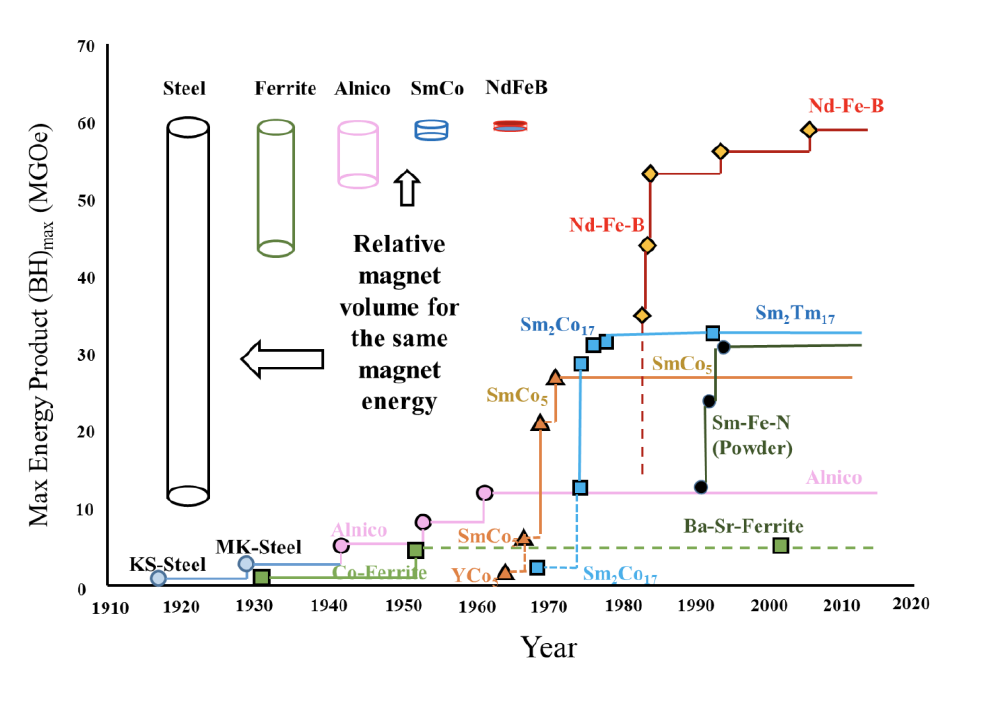
\includegraphics{fig/review/history.png}
	\caption[Development in energy product of permanent magnetic materials]{Development in energy product of permanent magnetic materials.}
	\label{fig:history}
\end{figure}

Nowadays, the rare-earth (REEs) FM became the most critical magnets in the market. Their dominating role might be explained due to their excellent magnetic properties at room temperature and their relatively low cost per energy-density unit. However, supply chain issues in recent years led to both prices and availability unpredictable issues.

The demand for hard magnetic materials becomes even bigger taking into account their numerous commercial applications in data storage, engines, actuators, generators, wind turbines, and hybrid cars. Not only increased demand but limited export from China has led to increased prices for these materials in the last years. These problems are forcing both industry and science to pay attention to the opportunities of developing new types of FM materials.

\section{Aim and Goals}

The ultimate goal of this study is to search for new technologically promising magnetic compositions. Considering the capabilities of modern evolutionary algorithms that allow identifying stable structures with a high magnetic moment, the problem of automated determination of the critical magnetic temperature (Curie point) remains unsolved. To solve the indicated problem and empower the end-user with a straightforward methodology for its calculation, the following research tasks are indicated:


\begin{enumerate}
\item Development and implementation of the critical magnetic temperature calculation methodology based on DFT approaches followed by Monte Carlo simulations.
\item Training of several classical ML models to solve a regression problem of critical temperature estimation based on the available experimental data.
\item Testing of the developed methods on compositions with known experimental and theoretical values of Curie temperature.
\item Computational search for new compositions with high magnetic properties using evolutionary algorithm USPEX.
\item Benchmarking of the newly find structures concerning their critical temperature to
determine the most promising from the technological viewpoint.
\end{enumerate}

\section{Outline}

Chapter 1 contains the current section with a problem background and formulation of the project objectives. Chapter 2 contains a general overview of the ferromagnetic materials properties and theoretical models used for this study. Chapter 3 describes the methodology used in this work, namely the construction of several machine learning (ML) models over available experimental data and calculations based on density function theory (DFT) followed by Monte-Carlo (MC) simulations. Chapter 4 is dedicated to the discussion of the results obtained by both methods. Finally, chapter 5 summarizes the research outcome and outlines possible future studies.



